
\section{Related Work}
Our work lies within the field of video understanding using language, specifically targetted towards the visual question answering task. We use spatio-temporal scene graphs to generate our questions, and provide a suite of new evaluation metrics to measure compositional reasoning.

%\noindent\textbf{Video understanding} Video understanding encompasses a large variety of tasks including action recognition \cite{fernando2016discriminative,song2016multimodal}, action localization~\cite{anne2017localizing,gao2017tall}, and future action prediction~\cite{nagarajan2020ego}, captioning~\cite{gan2017semantic,guadarrama2013youtube2text,venugopalan2015sequence,krishna2017dense}, commonsense understanding~\cite{park2020visualcomet}, and predicting social dynamics in movies~\cite{vicol2018moviegraphs}.  While all of these tasks require some form of compositional spatio-temporal comprehension, they do not explicitly measure anything beyond test set accuracy. Our work provides an explicit benchmark with metrics that explicitly measure generalization to longer videos, novel compositions, and indirect references to objects.

\noindent\textbf{Image Question answering benchmarks.}
A wide variety of visual question answering benchmarks have been created over the past five years~\cite{johnson2017clevr,hudson2019gqa,antol2015vqa,zellers2019recognition,goyal2017making,krishna2017visual,zhu2016visual7w,kim2020answering}. These benchmarks vary in input, from synthetic datasets~\cite{johnson2017clevr}, to cartoons~\cite{antol2015vqa}, to charts~\cite{kim2017deepstory}, to real-world images~\cite{hudson2019gqa,krishna2017visual,zhu2016visual7w,goyal2017making,zellers2019recognition,antol2015vqa}. They also vary in the type of questions asked, including descriptive (who, what, where, when, which, why, how)~\cite{zhu2016visual7w}, commonsense reasoning~\cite{zellers2019recognition}, spatial compositional reasoning~\cite{johnson2017clevr,hudson2019gqa}, and spatial localization~\cite{zhu2016visual7w,krishna2017visual,hudson2019gqa}. These benchmarks facilitated the development of many models architectures and learning algorithms explicit demonstrate spatial compositional reasoning abilities~\cite{lu2016hierarchical,vatashsky2020vqa,chen2020counterfactual}. However, none of these measure temporal reasoning beyond guessing common sense actions that usually require external knowledge~\cite{zellers2019recognition}. We are inspired from the work in spatial compositional reasoning and generalize to spatio-temporal compositional reasoning in videos.

\noindent\textbf{Video Question answering benchmarks.}
As we display in Table~\ref{tab:dataset_compare}, there is a growing interest in measuring the video reasoning capabilities using question answering~\cite{tapaswi2016movieqa,lei2018tvqa,jang2017tgif,kim2017deepstory,xu2017video,maharaj2017dataset,zeng2016leveraging,yu2019activitynet,yi2019clevrer}. Unfortunately, several of these prominent benchmarks rely on dialogue and plot summaries instead of reasoning over only the visual contents~\cite{lei2018tvqa,tapaswi2016movieqa,kim2017deepstory,zadeh2019social}, resulting in models with a stronger dependence on the dialogue input than on the visual input, reducing their effectiveness at measuring visual spatio-temporal reasoning~\cite{tapaswi2016movieqa,lei2018tvqa}.

Some video-only question-answering benchmarks are synthetically generated~\cite{yi2019clevrer, mun2017marioqa}, which affords the granular control necessary to measure model abilities like causality~\cite{yi2019clevrer}, or counting~\cite{mun2017marioqa}. However, they use short video clips, utilize only a handful of objects and lack the visual diversity of real-world videos. Furthermore, they do not focus on human object interaction and activities as we do. Other video-only question answering benchmarks suffer from biases and simplicity associated with human generated questions~\cite{yu2019activitynet,tapaswi2016movieqa,jang2017tgif,lei2018tvqa} or descriptions~\cite{xu2017video,zeng2016leveraging}. The largest human-annotated~\cite{lei2018tvqa} and generated~\cite{maharaj2017dataset} datasets contain $152.5K$ and $349K$ questions and refer to videos of less than $10$ seconds long. In comparison, our corpus is purely vision based, works on videos of $2-194$ seconds long, and evaluates complex and multi-step temporal reasoning.



% Many questions relevant to reasoning over videos require multi-step reasoning. A simple example covered by current datasets involves first localizing in time, then reasoning about that specific time. For example, this question from~\cite{jang2017tgif}, "What does the model do after lower coat?", requires finding when the model lowers her coat, then determining her activity after that. Another way to reason compositionally \mgm{is this a word?} is to refer to subjects indirectly, as the ImageQA benchmark~\cite{hudson2019gqa} does with "What color is the food on the red object to the left of the girl?". We use both temporal localization and indirect references to increase question compositionality, and we implement several metrics to measure different compositional reasoning abilities than existing Visual Question Answering benchmarks.

%Existing question-answering benchmarks are limited in the diversity of their questions. Since most benchmarks are image-based, they only test a model's reasoning over spatial relationships~\cite{johnson2017clevr,hudson2019gqa,antol2015vqa,goyal2017making,krishna2017visual,zhu2016visual7w}, object attributes~\cite{johnson2017clevr,hudson2019gqa, antol2015vqa,goyal2017making,krishna2017visual}, and common sense understanding~\cite{zellers2019recognition,antol2015vqa,krishna2017visual}. These benchmarks are unable to test reasoning over temporal relationships or activities beyond guessing based on common sense knowledge \cite{zellers2019recognition}. All questions asked by VideoQA benchmarks on non-synthetic videos that do not include extra textual information like dialogue limited temporal localization. Temporal localization refers to using the phrase "before/after/while $<$action$>$" to localize a relevant time in the video over which to reason. Questions in these benchmarks 1) can be answered from a single frame of the video, 2) apply to the entire video with no temporal localization, or 3) ask "what happened before/after/while $<$action$>$?"~\cite{jang2017tgif,xu2017video, maharaj2017dataset, zeng2016leveraging, yu2019activitynet}. Of the questions that apply to the entire video, some spatio-temporal topics are measured like counting and object and action recognition.


\noindent\textbf{Scene graphs.}
Scene graphs were first introduced as a Cognitive Science~\cite{biederman1982scene,wolfe1998visual} inspired representation for static images~\cite{krishna2017visual}. Each scene graph encodes objects as nodes in the image and pairwise relationships between objects as directed edges connecting nodes. 
%For example, an image with a \object{person} \relationship{throwing} \object{frisbee} would represent \object{person} and \object{frisbee} as nodes with a directed edge between them to represent \relationship{throwing}. 
The Computer Vision community has utilized the scene graph representation for a variety of tasks including visual question answering~\cite{johnson2017inferring}, relationship modeling~\cite{lu2016visual}, object localization~\cite{krishna2018referring}, evaluation~\cite{anderson2016spice}, generation~\cite{johnson2018image,ashual2019specifying}, retrieval~\cite{ashual2019specifying,johnson2015image}. Of particular interest to our project is how scene graphs from Visual Genome~\cite{krishna2017visual} were used by create GQA, a benchmark for compositional spatial reasoning over an image~\cite{hudson2019gqa}. Our work is a generalization of GQA's pipeline --- our pipeline develops templates that reason over not just objects and their relationships but also over how those relationships change over time to form different actions. We develop templates and programs that operate over Action Genome's recently released spatio-temporal scene graphs~\cite{ji2020action}.

\noindent\textbf{Compositional reasoning.}
While there are numerous definitions of compositionality, we in particular use what is more colloquially referred to as bottom-up compositionality --- ``the meaning of the whole is a function of the meanings of its parts''~\cite{cresswell1973logics}. In our case, reasoning about the question ``Was the person running or sitting for longer?'' requires finding the start and end of when the person was running and sitting, subtracting the start from the end, then comparing the lengths (Figure~\ref{fig:compo_fig}). Unfortunately, the most popular benchmarks and metrics defined to study compositional behavior have been limited to synthetic environments~\cite{keysers2019measuring,lake2018generalization,johnson2017clevr,yi2019clevrer} or to static images~\cite{hudson2019gqa}. Recent work has argued the importance of compositionality in enabling models to generalize to new domains, categories, and logical rules~\cite{lake2018generalization,vatashsky2020vqa} and have discovered that current models struggle with multi-step reasoning~\cite{fan2019heterogeneous}. These studies motivate a benchmark like ours that define multiple metrics to explore compositional reasoning in real-world videos.




\begin{figure*}[t]
    \centering
    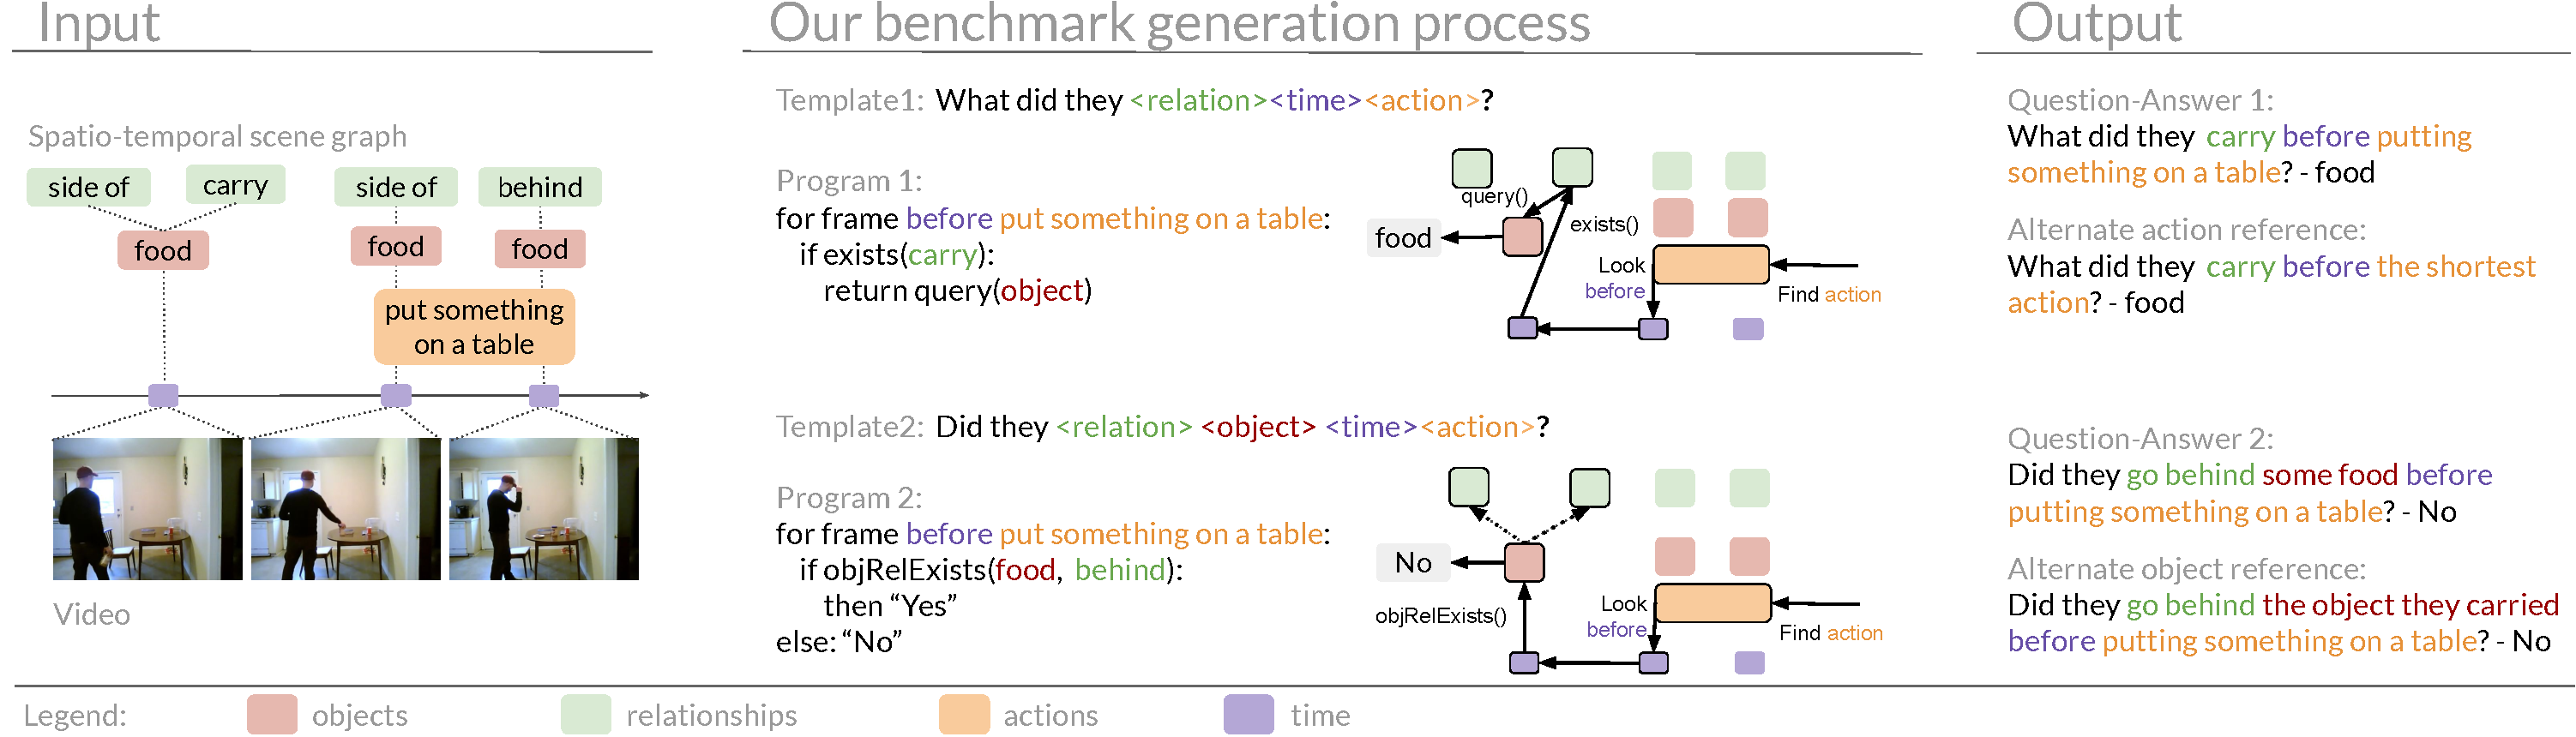
\includegraphics[width=0.95\linewidth]{figures/system.pdf}
    \caption{\textbf{Input:} To generate questions, we first ground the video in the \object{object}, \relationship{relation}, \action{action}, and \temporal{frame} level visual primitives by augmenting Action Genome's spatio-temporal scene graphs~\cite{ji2020action} and Charades' action annotations~\cite{sigurdsson2016hollywood}. \textbf{Our benchmark generation process:} we built a series templates with $<$tags$>$ that can be filled in with the associated primitive to generate a natural language question. Each template is also associated with a unique program that reasons over the spatio-temporal scene graph to automatically generate the answer to the question. \textbf{Output: } We create a dataset of question-answer pairs. Question diversity is increased by referencing primitives by their qualities (e.g. 'shortest action') or interactions (e.g. 'the object they carried').}
    \label{fig:system}
\end{figure*}